\documentclass[12pt, twoside]{book}
%\documentclass[12pt, oneside]{book}  % jednostranna tlac
\usepackage[a4paper,top=2.5cm,bottom=2.5cm,left=3.5cm,right=2cm]{geometry}
\usepackage[utf8]{inputenc}
\usepackage[T1]{fontenc}
\usepackage{graphicx}
\usepackage{url}
\usepackage[hidelinks,breaklinks]{hyperref}
\usepackage[english]{babel} % vypnite pre prace v anglictine
\usepackage{amsthm}
\usepackage{amsmath}
\usepackage{amsfonts}
\usepackage{enumerate}
\usepackage{algorithm}
\usepackage{algorithmic}
\usepackage{array}
\usepackage{booktabs}
%\usepackage{algorithm2e}
\usepackage{xcolor}
\usepackage{hhline}
\usepackage{pgfplots}
\usepackage{pgfplotstable}
\usepackage{listings}
\lstset{
  basicstyle=\ttfamily,
  columns=fullflexible,
  frame=single,
  breaklines=true,
  postbreak=\mbox{\textcolor{red}{$\hookrightarrow$}\space},
}
\usepackage{subfig}
%\usepackage{subcaption}
\usepackage{wrapfig}
\linespread{1.25} % hodnota 1.25 by mala zodpovedat 1.5 riadkovaniu

% -------------------
% --- Definicia zakladnych pojmov
% --- Vyplnte podla vasho zadania
% -------------------
\def\mfrok{2020}
\def\mfnazov{Identification of barcodes in nanopore sequencing data}
\def\mftyp{Master thesis}
\def\mfautor{Bc. Adri\'an Goga}
\def\mfskolitel{doc. Mgr. Tom\'a\v{s} Vina\v{r}, PhD.}

%ak mate konzultanta, odkomentujte aj jeho meno na titulnom liste
\def\mfkonzultant{doc. Mgr. Bronislava Brejov\'a, PhD. }  

\def\mfmiesto{Bratislava, \mfrok}

% bioinformatici odkomentujú riadok s dvoma odbormi
\def\mfodbor{ Computer Science}
%\def\mfodbor{ Informatika a Biológia } 
\def\program{ Computer Science }
% Ak je školiteľ z FMFI, uvádzate katedru školiteľa, zrejme by mala byť aj na zadaní z AIS2
% Ak máte externého školiteľa, uvádzajte Katedru informatiky 
\def\mfpracovisko{ Department of Computer Science }

\begin{document}     
\frontmatter


% -------------------
% --- Obalka ------
% -------------------
\thispagestyle{empty}

\begin{center}
\sc\large
Comenius University in Bratislava\\
The Faculty of Mathematics, Physics and Informatics

\vfill

{\LARGE\mfnazov}\\
\mftyp
\end{center}

\vfill

{\sc\large 
\noindent \mfrok\\
\mfautor
}

\cleardoublepage
% --- koniec obalky ----

% -------------------
% --- Titulný list
% -------------------

\thispagestyle{empty}
\noindent

\begin{center}
\sc  
\large
Comenius University in Bratislava\\
The Faculty of Mathematics, Physics and Informatics

\vfill

{\LARGE\mfnazov}\\
\mftyp
\end{center}

\vfill

\noindent
\begin{tabular}{ll}
Study programme: & \program \\
Field of study: & \mfodbor \\
Department: & \mfpracovisko \\
Supervisor: & \mfskolitel \\
Consultant: & \mfkonzultant \\
\end{tabular}

\vfill


\noindent \mfmiesto\\
\mfautor

\cleardoublepage
% --- Koniec titulnej strany


% -------------------
% --- Zadanie z AIS
% -------------------
% v tlačenej verzii s podpismi zainteresovaných osôb.
% v elektronickej verzii sa zverejňuje zadanie bez podpisov
% v pracach v naglictine anglicke aj slovenske zadanie

\newpage 
\thispagestyle{empty}
\hspace{-2cm}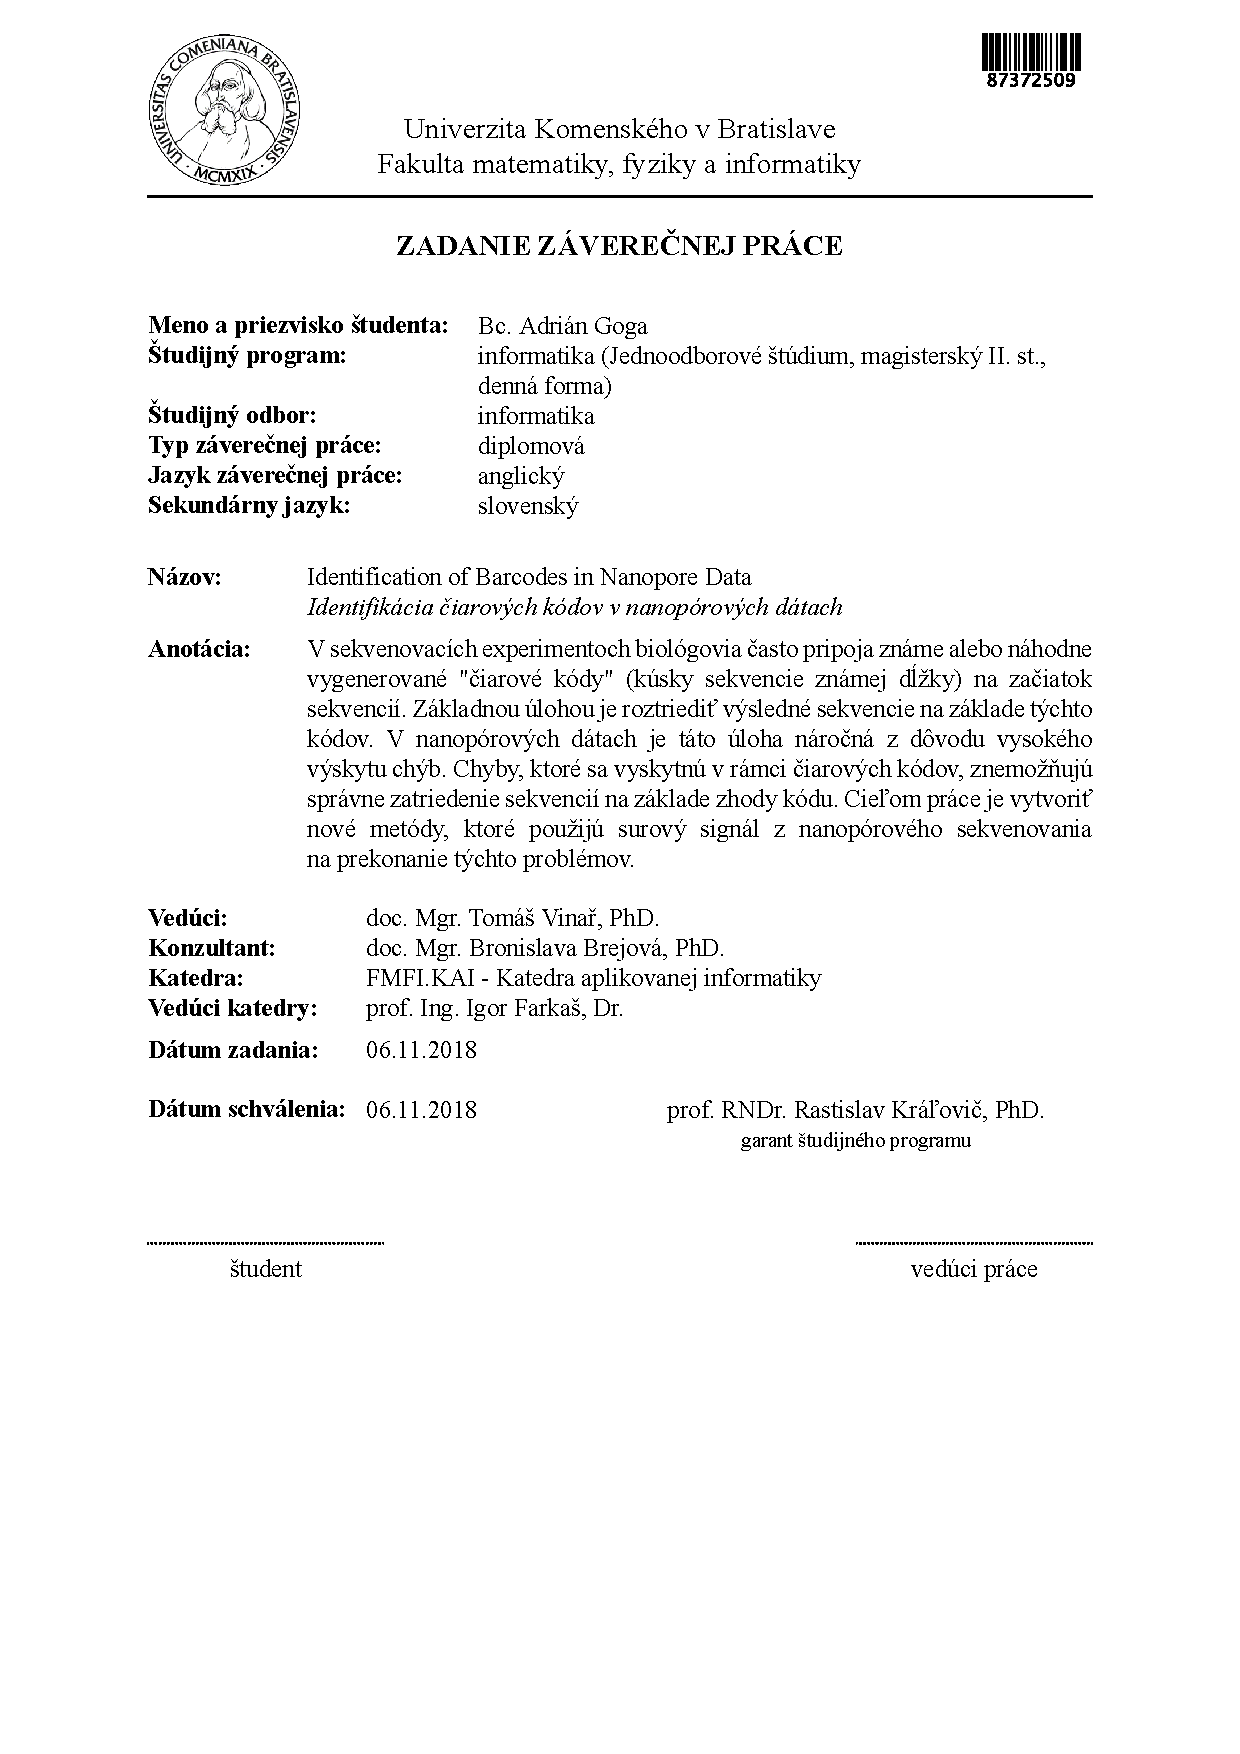
\includegraphics[width=1.1\textwidth]{images/zadanie_sk.PDF}
\newpage 
\thispagestyle{empty}
\hspace{-2cm}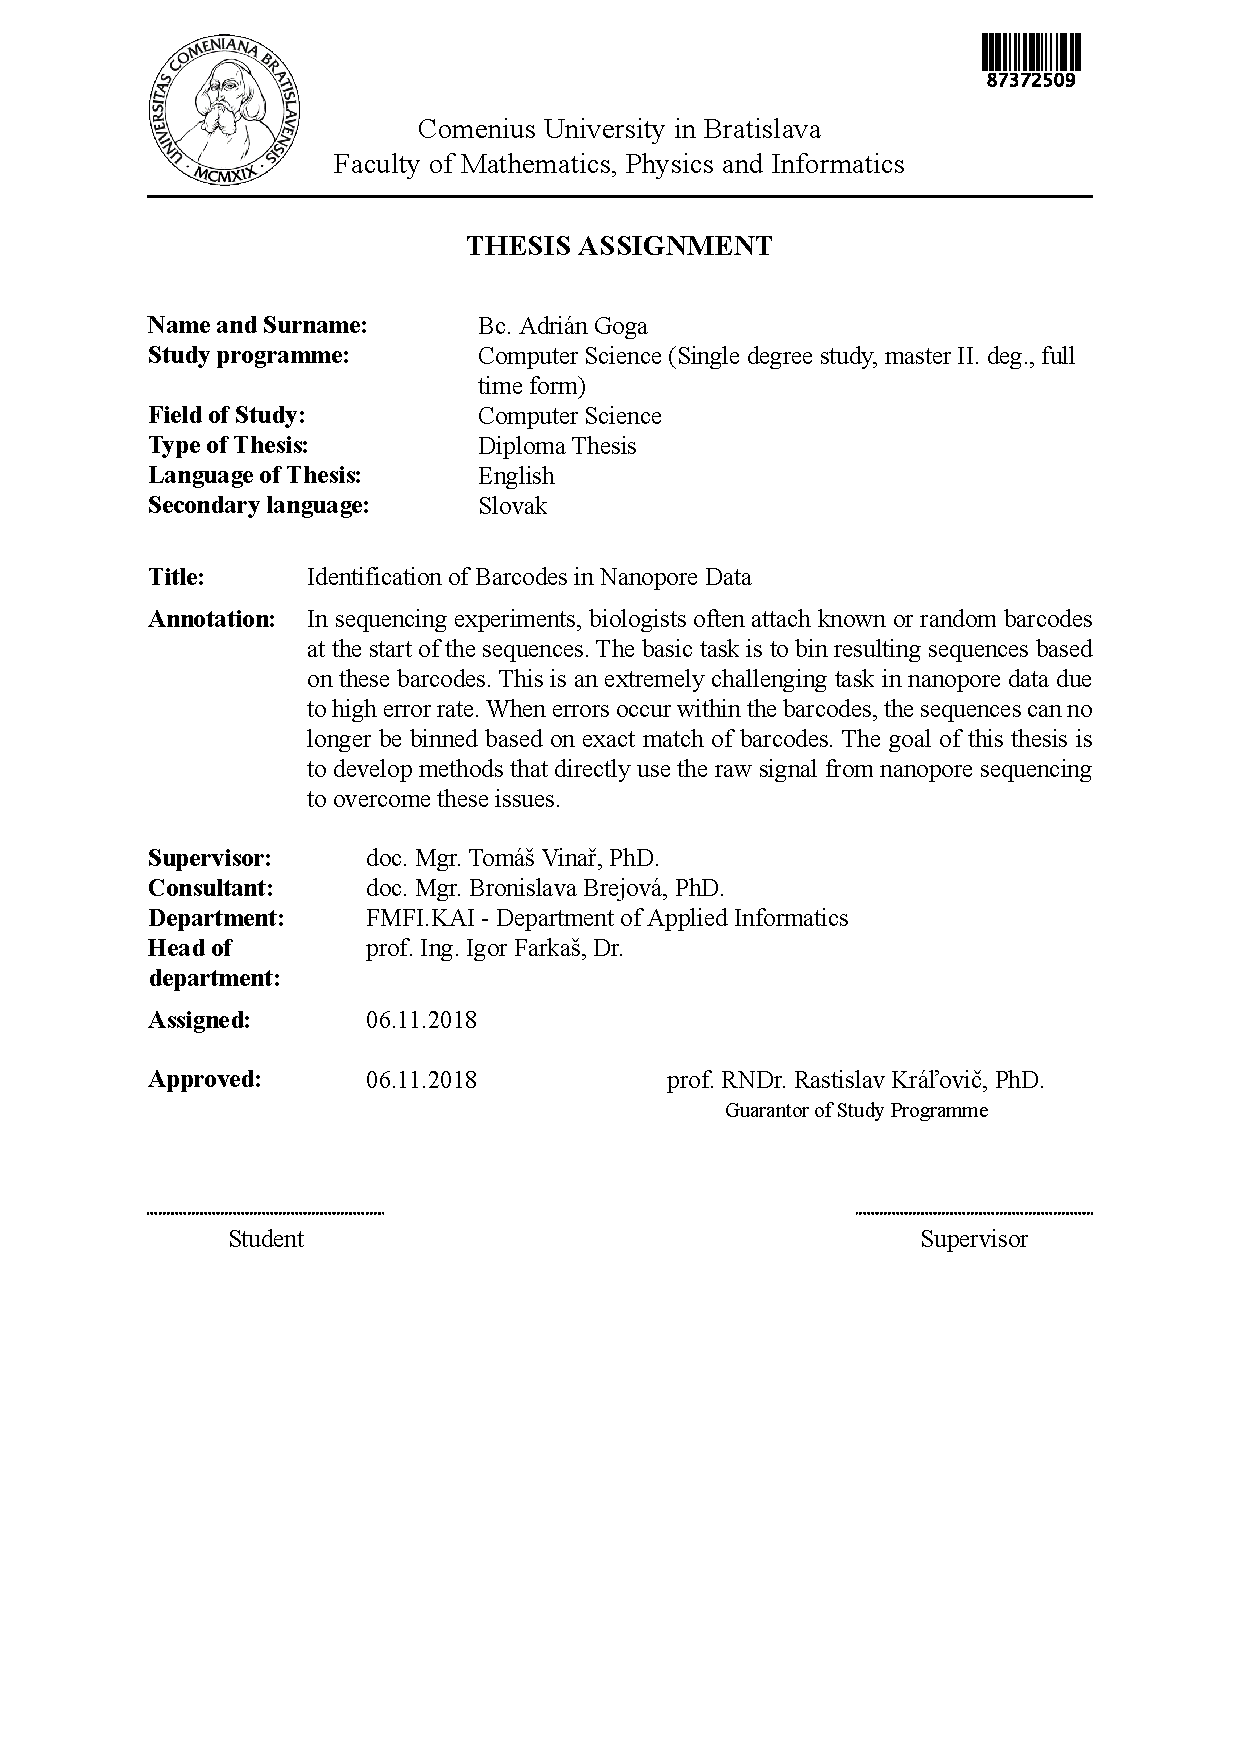
\includegraphics[width=1.1\textwidth]{images/zadanie_en.PDF}

% --- Koniec zadania

\frontmatter

% -------------------
%   Poďakovanie - nepovinné
% -------------------
\setcounter{page}{3}
\newpage 
~

\vspace{10cm}
\hspace{5cm}
\textit{Venovan\'{e} Maju\v{s}ke.}
\vfill

{\bf Acknowledgment:} I would like to thank my supervisor doc. Vina\v{r} for his unique guidance, an abundance of fruitful ideas and a portion of his precious time. No less thankful I am to doc. Brejov\'a, for helping me with anything when it was needed. Special thanks go to the members of my family, to whom I owe a lot.

% --- Koniec poďakovania

% -------------------
%   Abstrakt - Slovensky
% -------------------
\newpage 
\section*{Abstrakt}


Barkódovanie DNA sekvencií je metodológia v súčasnosti používaná v nanopórovom DNA sekvenovaní, ktorá umožňuje sekvenovanie niekoľkých genómov súčasne. Barkódovanie je ekonomicky výhodné, pretože na sekvenovanie je potrebná sekvenovacia komôrka, ktorej použitie je však jednorazové. Problém, ktorý barkódovaním vzniká je potreba tzv. debarkódovania, t.j. klasifikácia DNA čítaní podľa barkódu, ktorý obsahujú. Pôvodné prístupy k debarkódovaniu založené na zarovnávaní sekvencii po určení samotných DNA báz typicky nie sú schopné určiť barkód v $\approx 15\%$ prípadoch, kvôli chybám v preklade do reťazca nukleobáz. Nedávny prístup R. Wicka a spol. \cite{Deepbinner} v softvéri nazvanom Deepbinner, založenom na konvolučnej neurónovej sieti, ktorá spracováva surový signál zo sekvenovania, dosiahol doteraz najlepšiu úspešnosť v klasifikácii s chybovosťou iba  $\approx 1.6\%$ a $\approx 5.2\%$ stratou čítaní. My predstavujeme novú metódu debarkódovania, ktorá taktiež pracuje so surovým signálom, ale je na rozdiel od predošlých prístupov založená na učení bez učiteľa a teda nevyžaduje znalosť štruktúr sekvencií barkódov. Experimentálne výsledky ukazujú, že vo väčšine prípadov jej úspešnosť dokáže konkurovať Deepbinneru.

\paragraph*{Kľúčové slová:} DNA sekvenovanie, DNA barkódovanie, učenie bez učiteľa, zarovnávanie sekvencií, klasifikácia, analýza zhlukov
% --- Koniec Abstrakt - Slovensky


% -------------------
% --- Abstrakt - Anglicky 
% -------------------
\newpage 
\section*{Abstract}

DNA sequencing multiplexing is a technique that allows simultaneous sequencing of multiple genomes. This method is economically advantageous, since it uses a single-use flow cell to run several sequencing sessions. The challenge this method poses is demultiplexing, i.e. classifying the reads based on their barcode sequences. The original approaches based on aligning already basecalled sequences typically render up to $15\%$ of the reads unusable due to the errors in the basecalling process. The recent approach of Wick et al. \cite{Deepbinner} in a software called Deepbinner, which is based on a Convolutional Neural Network that operates with raw sequencing signal established a new state of the art with only $\approx 5.2\%$ of reads being unclassified and a $\approx 1.6\%$ error rate. We present a novel approach that also operates with raw sequencing signals. As opposed to the previous attempts at this problem, however, our method works in an unsupervised manner, i. e. without the preceding knowledge of the barcode sequences. Experimental results show that its performance is comparable to that of Deepbinner.


\paragraph*{Keywords:} DNA sequencing, DNA barcoding, unsupervised learning, sequence alignment, classification, clustering

% --- Koniec Abstrakt - Anglicky

% -------------------
% --- Predhovor - v informatike sa zvacsa nepouziva
% -------------------
%\newpage 
%\thispagestyle{empty}
%
%\huge{Predhovor}
%\normalsize
%\newline
%Predhovor je všeobecná informácia o práci, obsahuje hlavnú charakteristiku práce 
%a okolnosti jej vzniku. Autor zdôvodní výber témy, stručne informuje o cieľoch 
%a význame práce, spomenie domáci a zahraničný kontext, komu je práca určená, 
%použité metódy, stav poznania; autor stručne charakterizuje svoj prístup a svoje 
%hľadisko. 
%
% --- Koniec Predhovor


% -------------------
% --- Obsah
% -------------------

\newpage 

\tableofcontents

% ---  Koniec Obsahu

% -------------------
% --- Zoznamy tabuliek, obrázkov - nepovinne
% -------------------

\newpage 

\listoffigures
\listoftables

% ---  Koniec Zoznamov

\mainmatter

\input uvod.tex

\input intro_sequencing.tex

\input outline.tex

\input align.tex

\input data.tex

\input clustering.tex

\input zaver.tex

% -------------------
% --- Bibliografia
% -------------------


\newpage	

\backmatter

\thispagestyle{empty}
\nocite{*}
\clearpage

\bibliographystyle{plain}
\bibliography{literatura} 

%Prípadne môžete napísať literatúru priamo tu
%\begin{thebibliography}{5}
 
%\bibitem{br1} MOLINA H. G. - ULLMAN J. D. - WIDOM J., 2002, Database Systems, Upper Saddle River : Prentice-Hall, 2002, 1119 s., Pearson International edition, 0-13-098043-9

%\bibitem{br2} MOLINA H. G. - ULLMAN J. D. - WIDOM J., 2000 , Databasse System implementation, New Jersey : Prentice-Hall, 2000, 653s., ???

%\bibitem{br3} ULLMAN J. D. - WIDOM J., 1997, A First Course in Database Systems, New Jersey : Prentice-Hall, 1997, 470s., 

%\bibitem{br4} PREFUSE, 2007, The Prefuse visualization toolkit,  [online] Dostupné na internete: <http://prefuse.org/>

%\bibitem{br5} PREFUSE Forum, Sourceforge - Prefuse Forum,  [online] Dostupné na internete: <http://sourceforge.net/projects/prefuse/>

%\end{thebibliography}

%---koniec Referencii

% -------------------
%--- Prilohy---
% -------------------

%Nepovinná časť prílohy obsahuje materiály, ktoré neboli zaradené priamo  do textu. Každá príloha sa začína na novej strane.
%Zoznam príloh je súčasťou obsahu.
%
\addcontentsline{toc}{chapter}{Appendix A}
\input appendixA.tex
%\addcontentsline{toc}{chapter}{Appendix B}
%\input appendixB.tex
%\addcontentsline{toc}{chapter}{Appendix C}
%\input appendixC.tex
%
%\addcontentsline{toc}{chapter}{Appendix B}
%\input AppendixB.tex

\end{document}






